\documentclass[11pt,a4paper]{article}

%% ── Packages ──────────────────────────────────────────────────────────────────
\usepackage[T1]{fontenc}
\usepackage[utf8]{inputenc}
\usepackage[margin=2.2cm,top=2.4cm,bottom=2.6cm]{geometry}
\usepackage{lmodern}
\usepackage{microtype}
\usepackage[table]{xcolor}
\usepackage{amsmath}
\usepackage{amssymb}
\usepackage{graphicx}
\usepackage{array}
\usepackage{booktabs}
\usepackage{multirow}
\usepackage{tabularx}
\usepackage{enumitem}
\usepackage{parskip}
\usepackage{setspace}
\usepackage{titlesec}
\usepackage{fancyhdr}
\usepackage{fontawesome5}
\usepackage{tikz}
\usepackage[most]{tcolorbox}
\usepackage{calc}
\usepackage{hyperref}

\usetikzlibrary{positioning,calc,shapes.geometric,backgrounds,patterns}

%% ── Colour Palette ────────────────────────────────────────────────────────────
\definecolor{NavyDeep}{RGB}{15,32,66}
\definecolor{SlateBlue}{RGB}{42,78,140}
\definecolor{GoldAccent}{RGB}{196,155,63}
\definecolor{IceFog}{RGB}{237,242,250}
\definecolor{MidGray}{RGB}{108,117,135}
\definecolor{LightRule}{RGB}{214,221,234}
\definecolor{AlertRed}{RGB}{192,53,44}
\definecolor{SuccessGreen}{RGB}{38,128,88}

%% ── Hyperref ──────────────────────────────────────────────────────────────────
\hypersetup{
  colorlinks=false,
  hidelinks
}

%% ── Typography ────────────────────────────────────────────────────────────────
\renewcommand{\familydefault}{\sfdefault}

\titleformat{\section}
  {\color{NavyDeep}\large\bfseries}
  {}
  {0pt}
  {}
  [\vspace{2pt}\color{GoldAccent}\rule{\linewidth}{1.5pt}]

\titleformat{\subsection}
  {\color{SlateBlue}\normalsize\bfseries}
  {}
  {0pt}
  {}

\titlespacing{\section}{0pt}{18pt}{8pt}
\titlespacing{\subsection}{0pt}{12pt}{4pt}

%% ── Page Style ────────────────────────────────────────────────────────────────
\pagestyle{fancy}
\fancyhf{}
\fancyhead[L]{\textcolor{MidGray}{\footnotesize\textbf{CONFIDENTIAL} \textbar{} Meridian Advisory Partners}}
\fancyhead[R]{\textcolor{MidGray}{\footnotesize Business Restructuring Strategy Proposal}}
\fancyfoot[C]{\textcolor{MidGray}{\footnotesize\thepage}}
\fancyfoot[R]{\textcolor{MidGray}{\footnotesize\textit{Prepared for Nexa Holdings Group}}}
\renewcommand{\headrulewidth}{0pt}
\renewcommand{\footrulewidth}{0.4pt}
\renewcommand{\footrule}{\color{LightRule}\hrule width\headwidth height\footrulewidth}

%% ── tcolorbox Styles ──────────────────────────────────────────────────────────
\tcbset{
  execbox/.style={
    colback=NavyDeep!6,
    colframe=NavyDeep,
    fonttitle=\bfseries\small\color{white},
    coltitle=white,
    attach boxed title to top left={yshift=-2mm,xshift=6mm},
    boxed title style={colback=NavyDeep,colframe=NavyDeep,sharp corners},
    sharp corners,
    boxrule=0.6pt,
    top=8pt, bottom=8pt, left=10pt, right=10pt,
    title=#1
  },
  goldbox/.style={
    colback=GoldAccent!10,
    colframe=GoldAccent,
    sharp corners,
    boxrule=0.6pt,
    top=8pt, bottom=8pt, left=10pt, right=10pt
  },
  kpibox/.style={
    colback=NavyDeep,
    colframe=NavyDeep,
    sharp corners,
    boxrule=0pt,
    top=10pt, bottom=10pt, left=10pt, right=10pt,
    halign=center
  },
  alertbox/.style={
    colback=AlertRed!8,
    colframe=AlertRed,
    sharp corners,
    boxrule=0.6pt,
    top=6pt, bottom=6pt, left=10pt, right=10pt
  }
}

%% ── Helpers ───────────────────────────────────────────────────────────────────
\newcommand{\kpiblock}[2]{%
  \begin{tcolorbox}[kpibox]
    \textcolor{GoldAccent}{\large\bfseries #1}\\[2pt]
    \textcolor{white}{\footnotesize #2}
  \end{tcolorbox}%
}

\newcommand{\phaserow}[3]{%
  \textcolor{NavyDeep}{\textbf{#1}} & #2 & #3 \\
}

%% ══════════════════════════════════════════════════════════════════════════════
\begin{document}
\thispagestyle{empty}

%% ── Cover Block ───────────────────────────────────────────────────────────────
\begin{tikzpicture}[remember picture,overlay]
  \fill[NavyDeep] (current page.north west) rectangle
    ([yshift=-5.8cm]current page.north east);
  \fill[GoldAccent] ([yshift=-5.8cm]current page.north west) rectangle
    ([yshift=-6.08cm]current page.north east);
\end{tikzpicture}

\vspace*{0.3cm}
\begin{minipage}[t]{0.72\textwidth}
  \textcolor{white}{\footnotesize\textbf{MERIDIAN ADVISORY PARTNERS}
  \quad\textcolor{GoldAccent}{$\bullet$}\quad TURNAROUND \& RESTRUCTURING}\\[14pt]
  \textcolor{white}{\fontsize{26}{30}\selectfont\bfseries Business Restructuring}\\[2pt]
  \textcolor{white}{\fontsize{26}{30}\selectfont\bfseries Strategy Proposal}\\[10pt]
  \textcolor{GoldAccent}{\large\bfseries Prepared for Nexa Holdings Group}\\[6pt]
  \textcolor{white!80!NavyDeep}{\small
    Engagement Reference: MAP-2025-0874 \quad\textbar\quad
    Date: 14 November 2025 \quad\textbar\quad
    Version 2.1 — Final Draft}
\end{minipage}%
\hfill
\begin{minipage}[t]{0.25\textwidth}
  \raggedleft
  
\begin{tikzpicture}
    \fill[GoldAccent!20] (0,0) rectangle (3.2,3.2);
    \fill[GoldAccent] (0.15,0.15) rectangle (3.05,0.42);
    \draw[white,line width=1.2pt] (0.5,0.8) -- (2.7,0.8);
    \draw[white,line width=0.6pt] (0.5,1.15) -- (2.7,1.15);
    \draw[white,line width=0.6pt] (0.5,1.45) -- (2.1,1.45);
    \node[color=NavyDeep,font=\bfseries\large] at (1.6,2.3) {MAP};
    \node[color=NavyDeep,font=\tiny] at (1.6,1.95) {MERIDIAN};
    \node[color=NavyDeep,font=\tiny] at (1.6,1.75) {ADVISORY};
  \end{tikzpicture}
\end{minipage}

\vspace{3.4cm}

%% ── Confidentiality Notice ────────────────────────────────────────────────────
\begin{tcolorbox}[alertbox]
  \small\textcolor{AlertRed}{\faLock\enspace\textbf{Strictly Confidential.}}
  This document has been prepared solely for the management and board of Nexa Holdings Group.
  It contains commercially sensitive information and must not be disclosed to any third party
  without the prior written consent of Meridian Advisory Partners.
\end{tcolorbox}

\vspace{12pt}

%% ── Executive Summary ─────────────────────────────────────────────────────────
\section{Executive Summary}

Nexa Holdings Group (\textbf{``Nexa''} or the \textbf{``Company''}) is a diversified industrial
conglomerate with operations spanning precision manufacturing, logistics services, and specialty
chemicals. Following three consecutive years of declining EBITDA margins and a structural
deterioration in its legacy manufacturing segment, Nexa's board commissioned Meridian Advisory
Partners (\textbf{``Meridian''}) to conduct a comprehensive operational and financial review.

This proposal sets out a \textbf{24-month restructuring programme} designed to restore sustainable
profitability, rationalise the asset base, and position the Company for long-term value creation.
Our recommended strategy rests on three interdependent pillars:

\begin{itemize}[leftmargin=1.4em,itemsep=4pt]
  \item[\textcolor{GoldAccent}{\textbullet}]
    \textbf{Operational Transformation} — cost realignment, supply-chain consolidation, and
    manufacturing footprint rationalisation targeting \$38M in annualised savings.
  \item[\textcolor{GoldAccent}{\textbullet}]
    \textbf{Portfolio Simplification} — divestiture of two non-core divisions and redeployment
    of proceeds to strengthen the balance sheet.
  \item[\textcolor{GoldAccent}{\textbullet}]
    \textbf{Capital Structure Optimisation} — refinancing of existing senior debt facilities
    and introduction of a covenant-reset agreement with the lending syndicate.
\end{itemize}

\vspace{10pt}

%% ── KPI Strip ─────────────────────────────────────────────────────────────────
\noindent
\begin{minipage}[t]{0.23\textwidth}
  \kpiblock{\$38M}{Targeted Annual\\ Cost Savings}
\end{minipage}\hfill
\begin{minipage}[t]{0.23\textwidth}
  \kpiblock{18.4\%}{Pro-Forma EBITDA\\ Margin (Year 2)}
\end{minipage}\hfill
\begin{minipage}[t]{0.23\textwidth}
  \kpiblock{2.8$\times$}{Net Leverage\\ Target (Exit)}
\end{minipage}\hfill
\begin{minipage}[t]{0.23\textwidth}
  \kpiblock{24 Mo.}{Full Programme\\ Duration}
\end{minipage}

\vspace{14pt}

%% ── Situational Assessment ────────────────────────────────────────────────────
\section{Situational Assessment}

\subsection{Financial Performance — Current State}

Nexa's consolidated revenue of \$612M in FY2024 represented a 9\% decline from FY2022 peak
revenues of \$673M. EBITDA contracted from \$94M (14.0\% margin) to \$61M (10.0\% margin) over
the same period, driven primarily by input-cost inflation in the Precision Manufacturing segment
and volume erosion in Logistics Services.

\vspace{8pt}
\noindent
\begin{tabularx}{\linewidth}{@{}lXXXX@{}}
  \toprule
  \rowcolor{NavyDeep}
  \textcolor{white}{\textbf{Metric}} &
  \textcolor{white}{\textbf{FY2022}} &
  \textcolor{white}{\textbf{FY2023}} &
  \textcolor{white}{\textbf{FY2024}} &
  \textcolor{white}{\textbf{Variance}} \\
  \midrule
  Revenue (\$M)              & 673.1 & 638.4 & 612.2 & \textcolor{AlertRed}{$-9.1\%$} \\
  \rowcolor{IceFog}
  Gross Profit (\$M)         & 187.4 & 164.9 & 148.3 & \textcolor{AlertRed}{$-20.9\%$} \\
  EBITDA (\$M)               & 94.2  & 76.8  & 61.1  & \textcolor{AlertRed}{$-35.1\%$} \\
  \rowcolor{IceFog}
  EBITDA Margin (\%)         & 14.0\% & 12.0\% & 10.0\% & \textcolor{AlertRed}{$-400$\,bps} \\
  Net Debt (\$M)             & 198.0 & 231.5 & 274.3 & \textcolor{AlertRed}{$+38.5\%$} \\
  \rowcolor{IceFog}
  Net Leverage ($\times$)    & 2.1$\times$ & 3.0$\times$ & 4.5$\times$ & \textcolor{AlertRed}{$+2.4\times$} \\
  \bottomrule
\end{tabularx}

\vspace{12pt}

\subsection{Root-Cause Diagnosis}

\begin{tcolorbox}[goldbox]
\small
\begin{itemize}[leftmargin=1.2em,itemsep=3pt,topsep=2pt]
  \item[\lbrack 1\rbrack] \textbf{Fragmented manufacturing footprint:} Seven plants across four
    geographies operate below 62\% utilisation on average, generating \$22M in excess fixed cost.
  \item[\lbrack 2\rbrack] \textbf{Undifferentiated product portfolio:} Legacy SKUs face structural
    margin compression as low-cost Asian competitors capture commodity segments.
  \item[\lbrack 3\rbrack] \textbf{Debt overhang:} Acquisition financing from the 2021 Synapse
    Components transaction remains un-refinanced at a blended 7.8\% coupon; covenants breach
    is projected by Q2 2026 absent corrective action.
  \item[\lbrack 4\rbrack] \textbf{Talent and leadership gaps:} Three of five divisional CEO roles
    have been in interim tenure for more than 12 months, slowing strategic execution.
\end{itemize}
\end{tcolorbox}

\newpage

%% ── Proposed Organisational Structure ────────────────────────────────────────
\section{Proposed Organisational Structure}

The restructured entity will operate as a focused two-division holding company, shedding
non-strategic peripheral assets. The chart below illustrates the target operating model.

\vspace{10pt}

\begin{center}
\resizebox{\linewidth}{!}{%
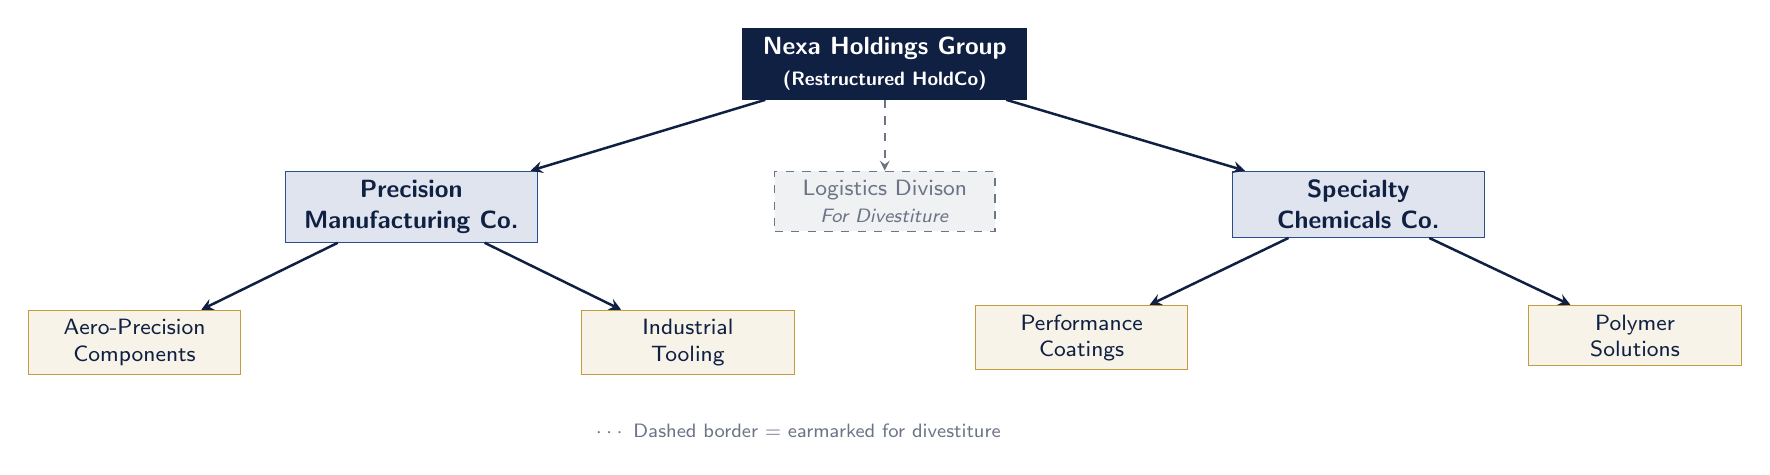
\begin{tikzpicture}[
  node distance=0.7cm and 1.1cm,
  box/.style={
    rectangle, draw=NavyDeep, fill=NavyDeep, text=white,
    minimum width=3.6cm, minimum height=0.80cm,
    align=center, font=\small\bfseries
  },
  divbox/.style={
    rectangle, draw=SlateBlue, fill=SlateBlue!15, text=NavyDeep,
    minimum width=3.2cm, minimum height=0.72cm,
    align=center, font=\small\bfseries
  },
  unitbox/.style={
    rectangle, draw=GoldAccent, fill=GoldAccent!12, text=NavyDeep,
    minimum width=2.7cm, minimum height=0.64cm,
    align=center, font=\footnotesize
  },
  divest/.style={
    rectangle, draw=MidGray, fill=MidGray!10, text=MidGray,
    minimum width=2.8cm, minimum height=0.64cm,
    align=center, font=\footnotesize,
    dashed
  },
  arr/.style={draw=NavyDeep, ->, >=stealth, line width=0.9pt},
  darr/.style={draw=MidGray, ->, >=stealth, dashed, line width=0.6pt}
]

%% Level 0 — HoldCo
\node[box] (hc) {Nexa Holdings Group\\{\scriptsize (Restructured HoldCo)}};

%% Level 1 — Core Divisions
\node[divbox, below left=0.9cm and 2.6cm of hc]  (pm) {Precision\\Manufacturing Co.};
\node[divbox, below right=0.9cm and 2.6cm of hc] (sc) {Specialty\\Chemicals Co.};

%% Level 1 — Divest
\node[divest, below=0.9cm of hc] (dv) {Logistics Divison\\{\scriptsize \textit{For Divestiture}}};

%% Level 2 — Business Units under PM
\node[unitbox, below left=0.85cm and 0.55cm of pm]  (pm1) {Aero-Precision\\ Components};
\node[unitbox, below right=0.85cm and 0.55cm of pm] (pm2) {Industrial\\ Tooling};

%% Level 2 — Business Units under SC
\node[unitbox, below left=0.85cm and 0.55cm of sc]  (sc1) {Performance\\ Coatings};
\node[unitbox, below right=0.85cm and 0.55cm of sc] (sc2) {Polymer\\ Solutions};

%% Arrows
\draw[arr] (hc) -- (pm);
\draw[arr] (hc) -- (sc);
\draw[darr] (hc) -- (dv);
\draw[arr] (pm) -- (pm1);
\draw[arr] (pm) -- (pm2);
\draw[arr] (sc) -- (sc1);
\draw[arr] (sc) -- (sc2);

%% Legend
\node[below=0.5cm of pm2, xshift=1.4cm, font=\scriptsize, text=MidGray]
  {$\cdots$ Dashed border = earmarked for divestiture};

\end{tikzpicture}
}%
\end{center}

\vspace{10pt}

%% ── Restructuring Pillars ─────────────────────────────────────────────────────
\section{Restructuring Pillars}

\subsection{Pillar 1 — Operational Transformation}

Meridian's operational review identified \textbf{\$38M} in annualised cost savings achievable
within 18 months. Key initiatives include:

\vspace{6pt}
\noindent
\begin{minipage}[t]{0.48\textwidth}
  \begin{tcolorbox}[execbox={Manufacturing Footprint}]
    \footnotesize
    Consolidate seven production sites to four, concentrating volume at the Harbridge
    and Eastmoor facilities (highest OEE\,/\,lowest unit cost). Estimated saving:
    \textbf{\$14.2M} p.a. Workforce reduction of approximately 340 FTEs with comprehensive
    transition support.
  \end{tcolorbox}
\end{minipage}\hfill
\begin{minipage}[t]{0.48\textwidth}
  \begin{tcolorbox}[execbox={Supply-Chain Consolidation}]
    \footnotesize
    Re-tender Tier-1 raw-material contracts (steel, specialty polymers) under a single
    group procurement framework. Move from 14 fragmented regional suppliers to a
    preferred panel of 5, unlocking volume rebates and payment term improvements.
    Estimated saving: \textbf{\$9.6M} p.a.
  \end{tcolorbox}
\end{minipage}

\vspace{8pt}
\noindent
\begin{minipage}[t]{0.48\textwidth}
  \begin{tcolorbox}[execbox={Overhead Rationalisation}]
    \footnotesize
    Centralise shared services (Finance, HR, Legal) into a single Group Services Centre
    in Veradene. Eliminate duplicate divisional back-office functions currently costing
    \textbf{\$8.4M} per annum. Target SLA-driven service delivery by Month 9.
  \end{tcolorbox}
\end{minipage}\hfill
\begin{minipage}[t]{0.48\textwidth}
  \begin{tcolorbox}[execbox={Digital \& Automation}]
    \footnotesize
    Deploy predictive-maintenance IoT across core production lines (capex: \$3.1M),
    projected to reduce unplanned downtime by 28\% and yield a maintenance-cost
    saving of \textbf{\$5.8M} p.a. Full payback within 6.4 months at current run-rate.
  \end{tcolorbox}
\end{minipage}

\vspace{10pt}

\subsection{Pillar 2 — Portfolio Simplification}

The Logistics Services division (\textbf{Nexalog}) and the Consumer Packaging unit will be
divested in a structured dual-track process (trade sale preferred; IPO fallback).
Combined indicative enterprise value range: \textbf{\$115M -- \$135M}, implying 6.5$\times$--7.5$\times$
FY2024 EBITDA. Net proceeds after tax and transaction costs of approximately \textbf{\$92M}
will be applied to debt reduction, bringing pro-forma net leverage below 3.0$\times$ at close.

\vspace{6pt}
\begin{tcolorbox}[goldbox]
\small
\textbf{Divestiture Timeline:} Vendor due-diligence pack targeted for completion by
28 February 2026 (Month 3). Process launch Q1 2026. Binding bids Q3 2026. Completion
subject to regulatory clearance, expected by Q4 2026.
\end{tcolorbox}

\vspace{10pt}

\subsection{Pillar 3 — Capital Structure Optimisation}

\begin{tcolorbox}[execbox={Debt Refinancing \& Covenant Reset}]
\small
Meridian has engaged Apex Capital Markets as financial adviser to manage a comprehensive
refinancing of Nexa's \$274M senior secured facility. The proposed structure comprises:
\begin{itemize}[leftmargin=1.2em,itemsep=2pt,topsep=4pt]
  \item \textbf{Term Loan B — \$160M} at Euribor\,+\,325\,bps, 5-year tenor, with 1\% annual
    amortisation and a springing covenant at 5.5$\times$ leverage.
  \item \textbf{Revolving Credit Facility — \$60M} at Euribor\,+\,275\,bps, providing
    working-capital flexibility through the transformation period.
  \item \textbf{Covenant holiday} for Q1–Q3 2026, stepping back in at amended levels aligned
    to the restructuring financial plan.
\end{itemize}
\end{tcolorbox}

\newpage

%% ── Implementation Roadmap ────────────────────────────────────────────────────
\section{Implementation Roadmap}

\vspace{4pt}
\noindent
\begin{tabularx}{\linewidth}{@{}>{\bfseries\color{NavyDeep}}p{2.6cm}Xp{3.8cm}@{}}
  \toprule
  \rowcolor{NavyDeep}
  \textcolor{white}{\textbf{Phase}} &
  \textcolor{white}{\textbf{Key Activities}} &
  \textcolor{white}{\textbf{Milestones \& Timing}} \\
  \midrule
  Phase 1\\{}[0pt] Stabilisation & %
    Appoint permanent divisional leadership; implement cash-preservation measures
    (freeze discretionary capex, extend payables); launch lender engagement process;
    establish Programme Management Office (PMO). &
    \faCalendar\enspace Jan -- Mar 2026\newline
    \textcolor{SuccessGreen}{\faCheckCircle}\enspace PMO live by Day 30\newline
    \textcolor{SuccessGreen}{\faCheckCircle}\enspace Interim CFO confirmed \\
  \midrule
  Phase 2\\{}[0pt] Transformation & %
    Execute plant consolidation; re-tender procurement contracts; launch Nexalog
    divestiture process; deploy shared-services centre; initiate IoT programme
    with Vertex Systems as technology partner. &
    \faCalendar\enspace Apr -- Oct 2026\newline
    \textcolor{SuccessGreen}{\faCheckCircle}\enspace Plant 3 closure by M6\newline
    \textcolor{SuccessGreen}{\faCheckCircle}\enspace Binding bids M9 \\
  \midrule
  Phase 3\\{}[0pt] Value Creation & %
    Complete divestitures and apply net proceeds to debt; launch premium product
    repositioning in Specialty Chemicals; invest in Aero-Precision growth capex;
    exit PMO with embedded continuous-improvement culture. &
    \faCalendar\enspace Nov 2026 -- Dec 2027\newline
    \textcolor{SuccessGreen}{\faCheckCircle}\enspace Net leverage $<$2.8$\times$\newline
    \textcolor{SuccessGreen}{\faCheckCircle}\enspace EBITDA margin 18\%$+$ \\
  \bottomrule
\end{tabularx}

\vspace{14pt}

%% ── Financial Projections ─────────────────────────────────────────────────────
\section{Financial Projections — Restructured Base Case}

\vspace{4pt}
\noindent
\begin{tabularx}{\linewidth}{@{}lXXXX@{}}
  \toprule
  \rowcolor{NavyDeep}
  \textcolor{white}{\textbf{(\$M)}} &
  \textcolor{white}{\textbf{FY2025E}} &
  \textcolor{white}{\textbf{FY2026E}} &
  \textcolor{white}{\textbf{FY2027E}} &
  \textcolor{white}{\textbf{CAGR}} \\
  \midrule
  Revenue (Continuing Ops.)   & 498.0 & 521.0 & 548.0 & \textcolor{SuccessGreen}{$+4.9\%$} \\
  \rowcolor{IceFog}
  Gross Profit                & 139.4 & 156.3 & 172.6 & \textcolor{SuccessGreen}{$+11.3\%$} \\
  Gross Margin                & 28.0\% & 30.0\% & 31.5\% & \textcolor{SuccessGreen}{$+350$\,bps} \\
  \rowcolor{IceFog}
  EBITDA (reported)           & 67.2  & 82.8  & 100.8 & \textcolor{SuccessGreen}{$+22.5\%$} \\
  EBITDA Margin               & 13.5\% & 15.9\% & 18.4\% & \textcolor{SuccessGreen}{$+490$\,bps} \\
  \rowcolor{IceFog}
  Net Debt (post-divest.)     & 260.0 & 178.0 & 128.0 & -- \\
  Net Leverage ($\times$)     & 3.9$\times$ & 2.1$\times$ & 1.3$\times$ & -- \\
  \bottomrule
\end{tabularx}

\vspace{10pt}

\begin{tcolorbox}[goldbox]
\small\textbf{Sensitivity note:} Projections assume a 2\% annual volume recovery in Precision
Manufacturing from H2 2026 and stable specialty-chemicals pricing. A 100\,bps margin shortfall
against plan reduces FY2027 EBITDA by approximately \$5.5M, which remains within covenant
headroom under the proposed refinancing terms.
\end{tcolorbox}

\vspace{14pt}

%% ── Risk Register ─────────────────────────────────────────────────────────────
\section{Key Risks \& Mitigations}

\vspace{4pt}
\noindent
\begin{tabularx}{\linewidth}{@{}p{3.2cm}p{1.4cm}p{1.4cm}X@{}}
  \toprule
  \rowcolor{NavyDeep}
  \textcolor{white}{\textbf{Risk}} &
  \textcolor{white}{\textbf{Impact}} &
  \textcolor{white}{\textbf{Likelihood}} &
  \textcolor{white}{\textbf{Mitigation}} \\
  \midrule
  Divestiture proceeds below plan &
    High & Medium &
    Dual-track process (trade/IPO); floor valuation set at 6.0$\times$; break-fee provisions. \\
  \rowcolor{IceFog}
  Lender covenant breach (pre-reset) &
    High & Low &
    Proactive engagement commenced; waivers pre-agreed; reset terms being documented. \\
  Key talent attrition during restructuring &
    Medium & Medium &
    Retention pool of \$3.8M approved; new LTIP scheme linked to restructuring KPIs. \\
  \rowcolor{IceFog}
  Execution delays in plant consolidation &
    Medium & Medium &
    PMO with weekly steering committee; contingency buffer of 6 weeks built into plan. \\
  Macro downturn compressing end-markets &
    High & Low &
    Downside scenario modelled at $-5\%$ volume; covenant headroom maintained above 1.2$\times$. \\
  \bottomrule
\end{tabularx}

\vspace{14pt}

%% ── Governance & PMO ──────────────────────────────────────────────────────────
\section{Governance \& Programme Management}

\subsection{Steering Committee Composition}

\begin{itemize}[leftmargin=1.4em,itemsep=4pt]
  \item[\textcolor{GoldAccent}{\faUser}] \textbf{Caroline Whitfield} — Chair, Non-Executive Director, Nexa Holdings Group
  \item[\textcolor{GoldAccent}{\faUser}] \textbf{David Ashmore} — Group CEO, Nexa Holdings Group
  \item[\textcolor{GoldAccent}{\faUser}] \textbf{Priya Nandakumar} — Group CFO (Interim), Nexa Holdings Group
  \item[\textcolor{GoldAccent}{\faUser}] \textbf{James Calloway} — Managing Director, Meridian Advisory Partners (Lead)
  \item[\textcolor{GoldAccent}{\faUser}] \textbf{Lena Baumann} — Director, Meridian Advisory Partners (Workstream Lead)
  \item[\textcolor{GoldAccent}{\faUser}] \textbf{Ravi Okafor} — Partner, Apex Capital Markets (Debt Advisory)
\end{itemize}

\vspace{8pt}
The Steering Committee will convene \textbf{bi-weekly} throughout Phase 1 and Phase 2,
transitioning to monthly cadence in Phase 3. A dedicated PMO dashboard will be maintained in
Meridian's secure data room, providing real-time visibility on initiative status, savings
realisation, and covenant headroom.

\vspace{12pt}

%% ── Next Steps ────────────────────────────────────────────────────────────────
\begin{tcolorbox}[execbox={Recommended Immediate Next Steps}]
\small
\begin{enumerate}[leftmargin=1.4em,itemsep=4pt,topsep=4pt]
  \item Board ratification of this proposal and approval of the PMO budget (\$1.4M) by
    \textbf{28 November 2025}.
  \item Execution of Meridian's engagement letter and data-room access protocols by
    \textbf{5 December 2025}.
  \item Appointment of Permanent Group CFO — shortlist of three candidates has been provided
    under separate cover; first-round interviews scheduled for \textbf{9 December 2025}.
  \item Commencement of lender presentation process with Apex Capital Markets no later than
    \textbf{12 January 2026}.
  \item Vendor due-diligence kick-off for Nexalog divestiture — Meridian to lead with
    support from Vertex Legal LLP, target completion \textbf{28 February 2026}.
\end{enumerate}
\end{tcolorbox}

\vspace{14pt}

%% ── About Meridian ────────────────────────────────────────────────────────────
\section{About Meridian Advisory Partners}

Meridian Advisory Partners is an independent restructuring and turnaround advisory firm
with 22 offices across 14 countries. Founded in 1991, Meridian has advised on over
\$480 billion of restructuring transactions across industrials, consumer, healthcare,
and real-estate sectors. Our dedicated turnaround team comprises 340 professionals,
including former CFOs, operational executives, and sector specialists.

\vspace{6pt}
\noindent
\begin{minipage}[t]{0.48\textwidth}
  \begin{tcolorbox}[goldbox]
  \footnotesize
  \textbf{Key Contact}\\[4pt]
  \textbf{James Calloway}\\
  Managing Director, Restructuring\\
  Meridian Advisory Partners\\[3pt]
  \faEnvelope\enspace j.calloway@meridian-adv.com\\
  \faPhone\enspace +44 20 7946 0382\\
  \faMapMarker\enspace 12 Aldgate Square, London EC3N 4BX
  \end{tcolorbox}
\end{minipage}\hfill
\begin{minipage}[t]{0.48\textwidth}
  \begin{tcolorbox}[goldbox]
  \footnotesize
  \textbf{Document Control}\\[4pt]
  Reference: MAP-2025-0874\\
  Prepared by: Lena Baumann, Director\\
  Reviewed by: James Calloway, MD\\
  Approved: Caroline Whitfield, NED Chair\\[3pt]
  \faPen\enspace Version 2.1 — Final Draft\\
  \faCalendar\enspace 14 November 2025\\
  \faFile\enspace 4 pages (excl.\ appendices)
  \end{tcolorbox}
\end{minipage}

\vspace{16pt}

\begin{center}
  \textcolor{LightRule}{\rule{0.5\linewidth}{0.4pt}}\\[6pt]
  \textcolor{MidGray}{\footnotesize
    \textit{This document is prepared in good faith on the basis of information provided by Nexa
    Holdings Group and publicly available data. Meridian Advisory Partners makes no representation
    or warranty as to the accuracy of projections, which are inherently uncertain. All figures
    are indicative and subject to confirmatory due diligence.}}
\end{center}

\end{document}
